\documentclass[12pt]{beamer}
\usetheme{EastLansing}

\usepackage[utf8]{inputenc}
\usepackage[T1]{fontenc}
\usepackage[french]{babel}
\usepackage{amsmath}
\usepackage{amsfonts}
\usepackage{amssymb}
\usepackage{graphicx}
\usepackage{comment}

\author{N. \bsc{Ribero-Rios} \and C.-A. \bsc{Romain} \and B. \bsc{Rouger}}
\title{Exposé d'Immunologie 5}
\subtitle{Mesure de l’activité cytotoxique des lymphocytes T par le test de relargage de Chrome}
\logo{
\includegraphics[width=0.1\linewidth]{logo.png}}
% \institute{}
\date{}
% \subject{}
% \setbeamercovered{transparent}
% \setbeamertemplate{navigation symbols}{}

\begin{document}
\maketitle


\begin{frame}
  \transuncover
  \tableofcontents
\end{frame}


\section{Principe}
\subsection{Principe général}
\begin{frame}
  \transuncover
  \frametitle{Principe général}
  
  \textbullet~ Définition de \textbf{test de cytotoxicité}\\
  \vfill
  \textbullet~ Quantification de la cytotoxicité des LT CD8 activés en fonction d'un agent pathogène
  
\end{frame}


\subsection{Mise en \oe{}uvre}
\begin{frame}
  \transuncover
  \frametitle{Mise en \oe{}uvre du test de cytotoxicité}

  \begin{minipage}{0.45\linewidth}
    \textbullet~ Mise en culture d'un nombre déterminé de cellules / confluence\\
    \textbullet~ Marquage des protéines cytoplasmiques des cellules cibles au $^{51}$Chrome\\
    \textbullet~ Infection des cellules cibles par un agent pathogène
  \end{minipage}
  \hfill
  \vline
  \hfill
  \begin{minipage}{0.45\linewidth}
    \textbullet~ Mise en contact des cellules cibles avec les cellules effectrices (LT CD8+ spécifiques)
      \begin{itemize}
      \item granzyme B
      \item perforine
      \end{itemize}
    \textbullet~ Mesure de la radioactivité du surnageant\\
    \textbullet~ Calcul du taux de lyse
  \end{minipage}
\end{frame}

 \begin{frame}
   \frametitle{Mise en \oe{}uvre du test de cytotoxicité}
	 \begin{figure}
       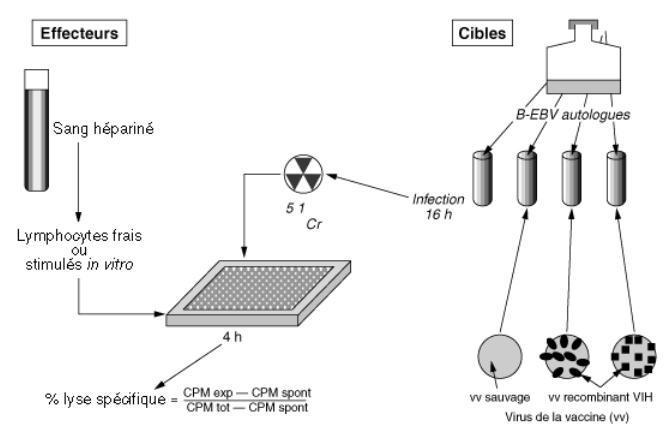
\includegraphics[width=0.7\linewidth]{presentation.png}
	 \end{figure}
  
 \end{frame}


\section{Avantages et inconvénients}
\subsection{Avantages}
\begin{frame}
  \transuncover
  \frametitle{Avantages}

  \begin{itemize}
  \item Technique la plus couramment employée
  \item Détection de la cytotoxicité
  \item Résultats reproductibles
  \item Le test le plus spécifique pour détecter la cytotoxicité cellulaire
  \item Facile à mettre en place
  \end{itemize}

\end{frame}


\begin{comment}
  \item Ne permet pas de détecter la mort cellulaire par apoptose
  \item Radioactivité (lourd à mettre en place, traitement des déchets, dangers lors de la manipulation)
  \item Besoin de lancer une culture de cellules cibles histocompatibles (long et lourd à mettre en place)
  \item Problème de virus à tropisme restreint
  \item Sensibilité faible
  \item Ne quantifie pas la production de cytokynes
  \end{itemize}

  \begin{center}
    \begin{tabular}{|p{0.4\linewidth} | p{0.4\linewidth} |}
      \hline 
      Avantages & Inconvénients \\ 
      \hline 
      \textbullet~ Le plus couramment employé & \textbullet~ Ne permet pas de détecter la mort par apoptose \\ 
                & \textbullet~ Utilisation de la radioactivité \\ 
      \hline 
    \end{tabular} 
  \end{center}

\end{frame}
\end{comment}
\subsection{Inconvénients}

\begin{frame}
  \transuncover
  \frametitle{Inconvénients}

  \begin{itemize}
  \item Ne permet pas de détecter la mort cellulaire par apoptose
  \item Radioactivité (lourd à mettre en place, nécessite un traitement des déchets, des précautions de manipulation)
  \item Besoin de lancer une culture de cellules cibles histocompatibles (lourd et long à mettre en place)
  \item Problème de virus à tropisme restreint
  \item Sensibilité faible
  \item Ne quantifie pas la production de cytokynes
  \item Besoin d'activer plusieurs fois les cellules effectrices (peut introduire un biais)
  \item Parfois de forts relargages spontanés de l'isotope radioactif
  \end{itemize}
\end{frame}


\section{Techniques complémentaires}
\subsection{Technique ELISPOT}

\begin{frame}
  \transuncover
  \frametitle{Technique ELISPOT (ENZYM LINKED IMMUNOSPOT)}
  
  \begin{itemize}
  	\item Détection des cellules effectrices et cellule mémoire produisant des cytokines au niveau cellulaire (dont TCD8+) $\rightarrow $ détection des cytokines ou des interleukines par des anticorps
  	\item Fixation des anticorps de capture puis saturation de la plaque (4\degres C une nuit)
  	\item Incubation des cellules avec stimulation par antigène. Les cytokines libérés sont captes par les anticorps. Incubation 6h-1 nuit
  	\item Lavage puis addition de l'anticorps de détection $+$ addition d'une enzyme de révélation (méthode biotine streptavidine) et révélation en ajoutant le substrat de l'enzyme
  \end{itemize}

\end{frame}

 \begin{frame}
 	\frametitle{Technique ELISPOT (ENZYM LINKED IMMUNOSPOT)}
 	\begin{figure}
 		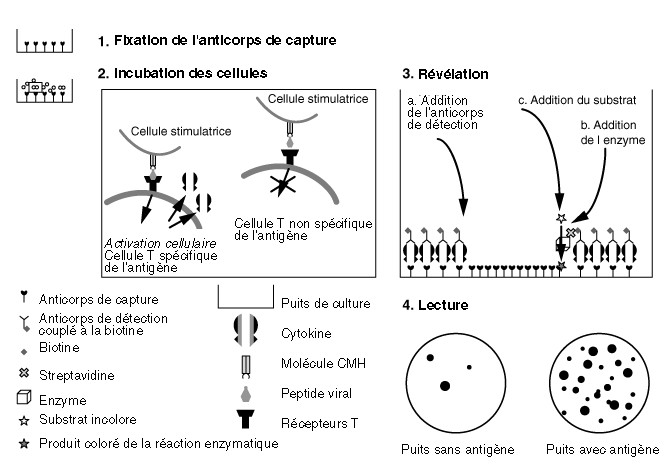
\includegraphics[width=0.7\linewidth]{elispot.jpg}
 	\end{figure}
 	
 \end{frame}

\begin{frame}
	\frametitle{Technique ELISPOT (ENZYM LINKED IMMUNOSPOT)}
	{\footnotesize
	\begin{tabular}{|p{0.45\linewidth}|p{0.45\linewidth}|}
		\hline
	Avantage & Inconvénients\\ 
	\hline
	\hline
	La plus utilisée après test de relargage au chrome & Pas d’estimation de cytotoxicité \\ 
	Utilisable pour toute molécule produite par LT CD8+ (cytokine, granzymes) &  Lecture essentiellement manuelle (lecture automatisée peu dévelloppée donc risque de variation de comptage entre différent expérimentateur)\\ 
	Plus sensible que relargage au chrome & Besoin d'avoir un épitope connus pour stimuler les lymphocytes \\ 
	Pas besoin de culture cible & On ne sait pas quelles cellules ont produit les cytokines \\ 
	Utilisable directement sur sang frais &  \\ 
	\hline
	\end{tabular} 
	}
\end{frame}

\subsection{Marquage intracellulaire des cytokynes}

\begin{frame}
  \transuncover
  \frametitle{Marquage intracellulaire des cytokynes}
  
  \begin{itemize}
  	\item Les LT CD8 sont activés \textit{in vivo}
  	\item Stimulation de cellule T in vitro avec monensine ou brefeldine A (bloquage du transport vésiculaire) incubation 6-15h
  	\item Incubation avec anticorps spécifique antigène de surface-fluorochrome
  	\item Lavage, fixation des cellules , perméabilisation+traitement anticorps spécifique au cytokine (cytométrie de flux)
  \end{itemize}

\end{frame}

\begin{frame}
	\frametitle{Marquage intracellulaire des cytokynes}
	{\footnotesize
		\begin{tabular}{|p{0.45\linewidth}|p{0.45\linewidth}|}
			\hline
			Avantage & Inconvénients\\ 
			\hline
			\hline
			Grand nombre de cellules analysées en même temps & Ne permet pas d’évaluer la cytotoxicité \\ 
			Utilisation de plusieurs anticorps avec différents fluorochromes Déterminer le phénotype des cellules (anticorps contre antigène de surface) &  \\
			\hline
		\end{tabular} 
	}
\end{frame}


\subsection{Technique de cytométrie}

\begin{frame}
  \transuncover
  \frametitle{Technique de cytométrie}
  
  \begin{figure}
  	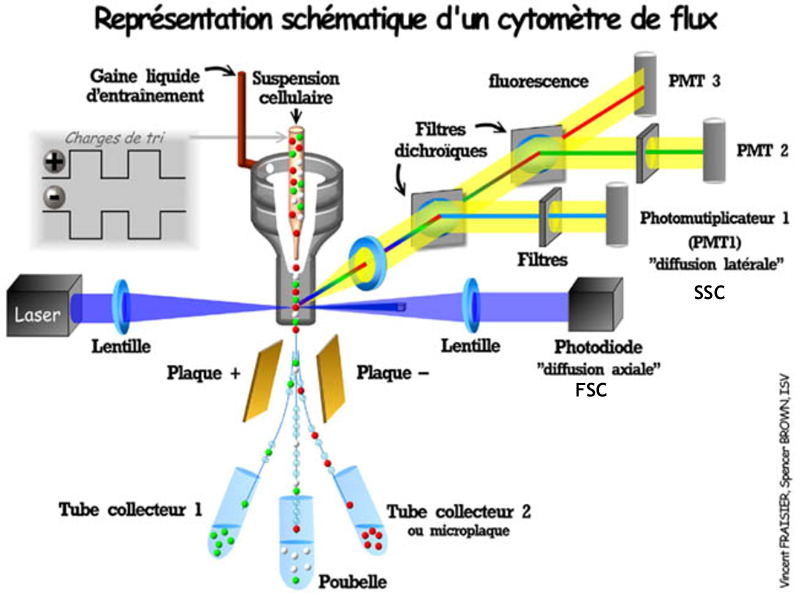
\includegraphics[width=0.7\linewidth]{cef.png}
  \end{figure}


\end{frame}

\begin{frame}
	\frametitle{Technique de cytométrie}
	{\scriptsize
\begin{tabular}{|p{0.45\linewidth}|p{0.45\linewidth}|}
	\hline
	Avantages & Inconvénients\\
	\hline
	\hline
	\textbullet~Possibilité de multi marquages & \textbullet~Coût de départ du cytomètre \\ 
	\textbullet~Rapide et peut être réalisé sur du sang frais ou cellule de moelle osseuse ou tumeur & \textbullet~Risque de chevauchement des spectres des fluorochromes \\ 
	\textbullet~+ sensible que le test au chrome (chaque cellule est passée) &  \\ 
	\textbullet~Gestion des déchets et protection du personnel manipulant moins lourd &  \\ 
	\textbullet~Possibilité de récupérer les cellules &  \\ 
	\textbullet~Possibilité de caractériser les cellules &  \\ 
	\textbullet~Monitorer la mort d’une cellule cible $ \rightarrow $ plus sensible que test au chrome &  \\ 
	\textbullet~Economie de réactifs quand plusieurs test en même temps sur l'échantillon & \\
	\hline
	
\end{tabular} 
}
\end{frame}

\section{Conclusion}

\begin{frame}
  \transuncover
  \frametitle{Conclusion}

	\textbullet~ Différentes techniques permettent l'évaluation de la spécificité des Lymphocytes T CD8$^+$. Une technique historique évalue une fonction de cytotoxicité : c'est la technique de relargage de l’isotope 51 du chrome.\\
	Elle tend à être remplacée par des techniques alternatives (Elispot, cytométrie) plus sensibles et plus rapides, et qui mesurent également d'autres fonctions ou marqueurs des lymphocytes T CD8+.\\
	
	
	\vfill
	
	\textbullet~ Technique de quantification sur la cytotoxicité et la sécrétion de cytokines : utile pour avoir une meilleure vue d’ensemble de la réponse immunitaire, une meilleure compréhension de la protection contre les pathogènes, de la réponse immunitaire des maladies auto-immunes et cancers, et pour produire de meilleurs vaccins.
	
	
\end{frame}

\appendix

\section{Références}

\begin{frame}
  \transuncover
  \frametitle{Références}

  \textbullet~ http://etudiantsfr.net/analyses-de-lymphocytes-t-specifiques-dantigenes/\\
  \vfill
  \textbullet~ Y. Rivière, F. Buseyne, D. Scott-Algara. Les outils d’exploration de l’activité des lymphocytes T CD8+. Virologie. 2000;4(6):463-71. (http://www.jle.com/fr/revues/vir/e-docs/les\_outils\_dexploration\_de\_lactivite\_des\_lymphocytes\_t\_cd8\_\_260033/article.phtml?tab=images)\\
  \vfill
  \textbullet~ New flow cytometric assays for monitoring cell-mediated cytotoxicity Liubov Zaritskaya1, Michael R Shurin2, Thomas J Sayers3, and Anatoli M Malygui,Expert Rev Vaccines. 2010 June ; 9(6): 601–616. doi:10.1586/erv.10.49.
\end{frame}

	
\end{document}